% #####################################################
% #####################################################
% #####################################################
\setchapterpreamble[u]{\margintoc}
\chapter{Vacuum RF Breakdown and Multipactor}\label{chap:Multipactor}

\epigraph{There is all the difference in the world between knowing about and knowing how to do.}{James Evans, The History and Practice of Ancient Astronomy}

\marginnote{Parts of this chapter are taken from \citeauthyear{hillairet2017} and from the PhD of Nicolas Fil and Adrien Plaçais and their associated publications \cite{fil2016, fil2017, fil2017-2,fil2018, placais2018,  placais2019}. These PhDs have been supervised in collaboration between CNES, ONERA and CEA since 2014.}

\section[RF Breakdowns]{RF Breakdowns and Vacuum Arcs}
RF breakdowns and vacuum arcs are a recurrent problematic in high RF power applications and magnetic nuclear fusion experiments make no exception. A \textit{vacuum arc} can be defined as an electric discharge occurring between two electrodes in vacuum \sidecite{Timko2011}. In the context of RF heating and current drive for tokamaks, electrical \textit{breakdown} almost always means a vacuum arc affecting RF systems performances. In this manuscript, both terms are used with the same meaning.

ICRH and LHRF systems have general concerns with voltage limitations, in particular \sidecite{bobkov2003, goniche2014}:
\begin{itemize}
	\item between metallic electrodes of coaxial lines,
	\item between waveguide walls of (thin) rectangular waveguides,
	\item with dielectric elements of vacuum feed-throughs,
	\item inner conductor mechanical supports
\end{itemize}
These parasitic phenomenon can limit the power transmitted from the RF sources to the plasma.

\subsection{Formation Mechanisms}

Despite the enormous number of papers published on this topic, some uncertainty remains about breakdown overall processes. This uncertainty is due to the fact that few mechanisms are (or seem) to be involved \sidecite{insepov2011-1}. Moreover, they occur on very short time scales \sidecite[+0.5cm]{zhou2019}, during which experimental parameters vary over 12 orders of magnitude \cite{Timko2011}. As setup are often unique and results delicate to compare for an application to another, few dedicated experimental studies have been conducted to explore different  experimental parameters relevant to tokamak antennas \sidecite{bobkov2003, Graves2006a, becerra2007, dinca2009}.

It is know since some time that DC breakdown mechanism under ultra-high vacuum is related to local breakdown fields which mostly depend on the electrode materials \sidecite{alpert1964, descoeudres2009}. Recent experimental and modelling works performed for accelerators argue that arcing can be explained by the properties of surface cracks and \textit{unipolar arcs}\sidenote[][+1cm]{unipolar arcs (or cathodic arcs) are similar to vacuum arcs, only instead of striking between two solid electrodes they strike between one solid electrode and a plasma\cite[§9.8]{wesson2011}.} and explained from the following steps \sidecite{insepov2013}:
\begin{enumerate}
\item An initial mechanical failure/cracks of the surface due to fatigue, producing detached fragments,
\item high external electric field is applied, locally enhanced at the failure/cracks location (known as \textit{emitters})
\item Electrons extracted from secondary or field emission further ionize these fragments,
\item A local plasma is initiated, controlled by the plasma sheath and material properties. 
\item The plasma density increases exponentially up to some equilibrium state, during which local temperature increases due ion bombardment/current hitting the wall, eventually melting it. Ion induced sputtering is a source of additional ions for the plasma.
\item Additional surface damages are produced by the arc (due to heating, melting then cooling), which can further initiate new arcs.
\end{enumerate}
If the energy source that gave birth to the arc is not stopped, the arc can continuously burn. Unipolar arcs can travel on the surfaces of the cathode (negatively charged), as the emitter spot is constantly changing. In the absence of a magnetic field, the spot "movement" can be described with a random-walk model\sidecite{daalder1983}. In the presence of a magnetic field $\Bbf_0$, the spot follows a retrograde motion in the $-\jbf\times\Bbf_0$ direction\sidecite{wesson2011}. 

As noted in the step 3, both field emission and secondary emission have been identified as the main mechanism leading to increase the electron population, which further cause ionization and electron avalanche \sidecite{hohn1997}. The leading cause depends of the geometry and the RF frequency at play. 

It is generally admitted in the fusion community that \textit{field emission} is the main mechanism limiting ICRF power while it is mostly  \textit{secondary emission} triggered by \textit{multipactor} effect for LHRF \sidecite{goniche2014, wukitch2004}. Field emission is an electron tunnelling effect induced by an electric field. Secondary emission is a phenomenon where primary incident particles of sufficient energy, when hitting a surface or passing through some material, induce the emission of secondary particles, mostly electrons called \textit{secondary electrons}. However, multipactor also affect ICRF systems, generally at relatively low power/voltage, but can also lead to breakdowns. Work on multipactor for ICRF and LHRF are detailled in Section~\ref{sec:multipactor_icrf} and Section~\ref{sec:multipactor_lhrf}. Because multipactor is affecting satellite payloads, a collaboration between CNES and ONERA has been initiated in 2004 and some results are presented in the next Sections.



\subsection{Arc Detection}
Breakdowns appearing in RF system can induce changes on the effective impedance which may detune the matching system and allows reflected power to return to the RF sources. Thus, reflection coefficient is the primary breakdown detection method in both ICRF and LHRF. However, if the breakdown is close to a voltage node, the VSWR or reflection coefficient’s phase may be almost unperturbed while increasing the apparent power coupling \sidecite{monakhov2007, goniche2014}. It is thus of great importance to detect these breakdowns as well as to switch-off sources fast enough to avoid damages. 

However, some kind of arcs do not change the reflection coefficient and can nevertheless damage components. Such arcs may arise in location of low voltage nodes and/or on vacuum feed-through \sidecite{baity2005, dinca2011-1}. The formation mechanisms of such arcs are complex and certainly multifactorial (geometry, materials) and are attributed to multipactor (or a consequence of a multipactor-initated discharge) \sidecite{monakhov2007, kishek1998}. 

Therefore, detection only based on reflection coefficient is not reliable enough to insure the safety of the system and additional detection techniques have been developed. Among these methods, we can list Sub-Harmonic Arc Detection (SHAD) \sidecite[-0.5cm]{dinca2011}, Scattering Matrix Arc Detection (SMAD) \sidecite{vrancken2009} or optical detection have been proposed or implemented in various systems, such as the WEST ICRH antenna, to complete reflection coefficient method \sidecite{dinca2009, bosia2011}. 



% #######################################################
\section[Multipactor]{Multipactor in High Power RF Devices}
Multipactor is a process by which electron population increases from a resonant \textit{secondary emission} multiplication inside an RF device operating under vacuum conditions. It was first recognized and described by \citeauthyear{farnsworth1934} for the purpose of electron multiplication in vacuum tubes. The electron population increases if both criteria are met\sidecite{vaughan1988}: 
\begin{itemize}
	\item A Secondary Emission Yield (SEY)\sidenote{The SEY is the number of secondary electrons emitted per incident electron impacting a material surface.} higher than one,
	\item A synchronism of the electron motion between a single  or two electrodes with the RF electric field.
\end{itemize}

In high power RF devices under vacuum, this phenomenon is usually not desirable, since it can detune RF systems or ultimately lead to an avalanche effect and the development of a discharge which can damage RF components, even at pressures two order of magnitude below Paschen breakdown limit \sidecite[-1cm]{kishek1998, graves2006}. As it concerns RF system in vacuum environment, it affects satellite payloads\sidecite{rozario1994, anzahormigo2014}, particle accelerators \sidecite[+0.7cm]{elkhaldi2019} and of course fusion experiments. When not detected quickly enough, local plasma can be initiated by multipacting electrons and finally to an arc \sidecite[-0.3cm]{hohn1997}. These arcs can lead to surface erosion \sidecite{goniche2012}, dielectric components metallization \sidecite{wang2015} or water/air leaks due to punctured components such as bellows or vacuum windows \sidecite{neuber1998, neuber2007}. 

%The ICRF and LHRF antennas are  made of copper or silver-coated stainless-steels structures and are located in vacuum environments. The vacuum sealing with pressurized transmission lines is made with the help of ceramics such as alumina, aluminium nitride, beryllium oxide or diamond. 

Signature of multipactor breakdowns have been found to be low amplitude and wideband spectrum of excited frequencies at the opposite behaviour than high voltage arcs \cite{dinca2009}. Voltage handling limits also arise in the antenna facing the plasma, which also reduce the power coupled by the antenna. Impurity production, increasing the neutral particles pressure, degrades the antenna voltage handling. Experimental works identified multipactor as the leading explanation for observed ICRF antenna neutral pressure limit \cite{graves2006}.

In some cases however, multipactor-induced discharges can be desired for vacuum RF conditioning \sidecite{mishra2010}. In addition to standard cleaning procedures, surface conditioning is necessary to increase the voltage handling capability. To this end, short low power (1-10~kW) RF pulses (100-1000~ms) are applied on RF antennas under vacuum (no plasma) to reduce the secondary emission of the metallic surfaces\sidecite{halbritter1982}. This method, used both in ICRF \sidecite[+0.5cm]{colestock1985, wang2015} and LHRF \sidecite[+1.5cm]{ekedahl1998,goniche2012} is an essential preliminary step before increasing both power and duration to medium values (10-100~kW/100-200~ms) in order to increase the surface temperature due to RF losses and make them out-gass (still in vacuum). Once done, RF commissioning on plasma at medium powers and durations can be realized to clean parts of the antenna that do not carry a substantial fraction of the current \sidecite{noterdaeme1993}, before finally achieved high voltage conditioning at high power (>100kW/10ms) to further increase the voltage stand-off limit. Hence, multipactor can depend on the operating conditions and its predictability is hence subject to the changes  in secondary emission properties of material. This aspect has been investigated in the frame of the PhD of Nicolas Fil and is reported in Section~\ref{sec:multipactor_TEEY}.

In addition, magnetic fusion RF heating and current drive systems are subjected to the high magnetic field environment of the experiments in the Tesla range. The presence of magnetic field affects obviously the electron trajectories and thus the multipactor resonances. During the PhD of Nicolas Fil \sidecite{fil2017-1}, he has measured that magnetic field also modify the secondary emission characteristics of a metal, which further impact multipactor processes (cf.Section~\ref{sec:multipactor_magnetic_field}). 

Finally, dielectric are also subject to multipactor, which can be critical when these dielectric are safety components such as vacuum feed-through/windows. Because they are not conductor per definition, dielectrics can accumulate electric charges at their surface. The dynamics of this accumulation can further modify multipactor discharges \sidecite{sorolla2017}. This aspect has been studied during the PhD of Adrien Plaçais \sidecite{placais2020} and develloped in Section~\ref{sec:multipactor_dielectric}.


\subsection{Multipactor in coaxial geometries}\label{sec:multipactor_icrf}
In coaxial geometries, multipactor-induced breakdown disappear when the power level is above few kilowatts \sidecite[-0.5cm]{woo1968, woo1970}, which is a typical signature of multipactor resonance as expected from theory  \sidecite{udiljak2007, semenov2007, becerra2007}. The later exact power level depends on the RF system such as $Q$-factor and transmission line dimensions and the materials used. Experimental 

The Figure~\ref{fig:powerthresholdcoax} illustrates the multipactor power threshold versus the line impedance as calculated in a coaxial geometry with a fixed outer diameter at 50~MHz \sidecite{hillairet2017}. Such breakdowns are known to happen when the power builds up during the start-up phase of the generators. For this reason, the RF rise time is generally set as short as possible, in order to exceed this power window as fast as possible (“push-through”) and to be faster than the multipactor rise time \sidecite{graves2006, kishek1997, baity2005, mishra2010}. In practice, the maximum current drawn by the generator or the RF power feedback systems limits this rise time to no more than typically 50~µs/kW, which is generally sufficient to avoid multipactor during power ramp-up. 

\begin{figure}[h]
	\centering
	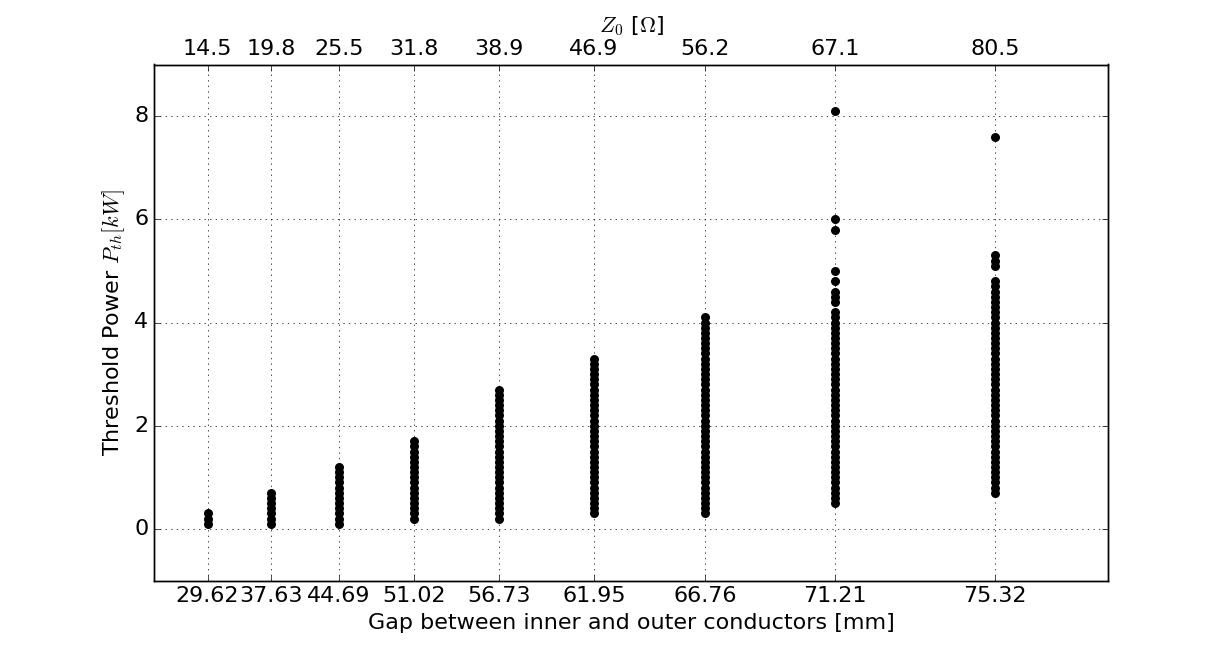
\includegraphics[width=1.0\linewidth]{figures/chap4/power_threshold_coax}
	\caption{Power Threshold in a coaxial line at 50 MHz calculated with Spark3D versus gap between inner and outer electrodes (with fixed outer diameter 153 mm) (Spark3D ECSS Copper SEY definition).}
	\label{fig:powerthresholdcoax}
\end{figure}




\subsection{Multipactor in rectangular waveguides}\label{sec:multipactor_lhrf}

%Vacuum arcs have been an experimental concern since the late 1970's \sidecite{ohkubo1977,timberlake1982}. Not only arcs can damage the components itself, but also they can release metallic impurities into the plasma (thus reducing the fusion power). While most arcs induce an increase of the reflected power, it some case however it can also remains unchanged or even decreases it.

%The physical mechanism leading to these arcs is attributed to gas waveguide wall out-gassings, multipactor or photoelectron emission.

%While the exact mechanism leading ultimately to arcs is barely fully certain, 

We have seen that in coaxial lines, multipactor appear above a certain lower electric field threshold, then disappear above an upper threshold. At the contrary, multipactor in rectangular waveguides is triggered only above a certain (large) electric field threshold \sidecite{semenov2007-1}. This has been early identified as a power-limiting mechanism in LHRF grill antennas \sidecite{hwang1981, vaughan1982, dobbing1997, goniche2012-2, goniche2014}. 


Various strategies have been tested to improve power limits in LHRF grill antennas. Surface treatment to decrease electron secondary emission has been tested in various experiments \sidecite[+0.5cm]{timberlake1982}. However, because of further surface changes appearing during component's life, such as chemical reactions with present species or surface erosion/deposition. Hence, such solution might be inherently less reliable on the long-term. For example, carbon layer had been deposited on JET prototype L0 launcher but was gave up in later prototypes due to its tendency to flake-off \sidecite{dobbing1997, ekedahl1998}.

Changing the antenna material itself had also been investigated. Because of its low secondary emission yield, titanium has been used on JFT-2, Versator II, WEGA and Petula-B \sidecite{england1989}. However, after an initial period of successful operation, titanium surface is rapidly altered, increasing its secondary emission yield. On the Alcator C-Mod tokamak, chemical reactions between deuterium and a titanium grill antenna has been observed, which created a brittle titanium deuteride compound. The antenna disintegrated into titanium deuteride dust and the LH launcher was finally removed from the tokamak\cite{wallace2010}. 

Modification of the waveguide shape has also been proposed. From the experience acquired on vacuum tubes, it has been suggested that making each of the LH grill dividing septa thicker in the middle than at the edge, in order to introduce a slight lateral component of the electric field which in returns modify electron trajectories, might lead to multipactor suppression \sidecite{vaughan1982}.

Multipactor had also been associated in the LHRF with window failures \sidecite{ikeda1989}. Discharges at pillbox windows at a pressure below $10^{-2}$~Pa which produces no or little effect on the reflected power have been observed. During these discharges, large temperature rise was also monitored, about 100 times higher than that in a no-discharge case at the power level of 500~kW. The discharges can be suppressed by sufficient RF conditioning and/or by a thin coating (around 10~nm) of Titanium Nitride (TiN) which has a lower secondary emission yield than the ceramic \sidecite{suharyanto2007, kaabi-1}. The later method is widely used on high power RF windows, for example on WEST 3.7~GHz windows \sidecite{peauger2005} or 5~GHz windows \sidecite[+0.5cm]{hillairet2015, kim2019-2} (cf. Section~\ref{sec:RF_windows}).


A peculiarity of LHRF antenna with respect to satellite payloads is that they usually operate with a non negligible SWR inside the launcher due to the plasma medium which reflects between 20 to 50\% of the input power. Hence, multipactor threshold in terms of power is not relevant and should instead be formulated in terms of electric field threshold then linked to a given power input and reflection coefficient. 

\begin{marginfigure}[-1cm]
	\centering
	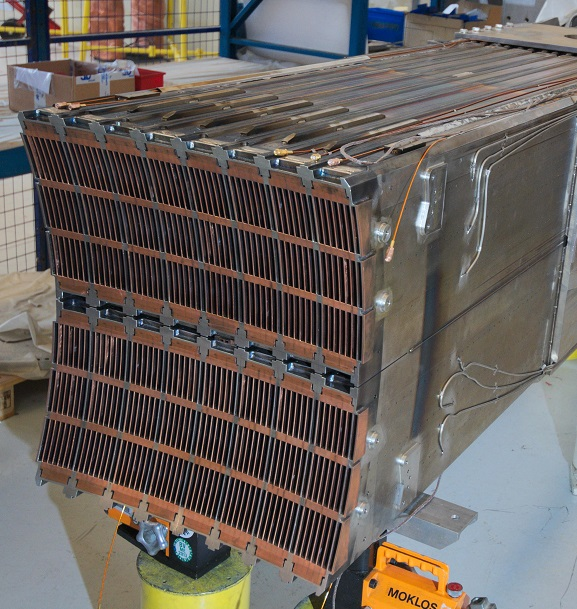
\includegraphics[width=0.9\linewidth]{figures/chap4/WEST_LH1}
	\caption{WEST LH1 antenna}
	\label{fig:westlh1}
\end{marginfigure}

\begin{marginfigure}
	\centering
	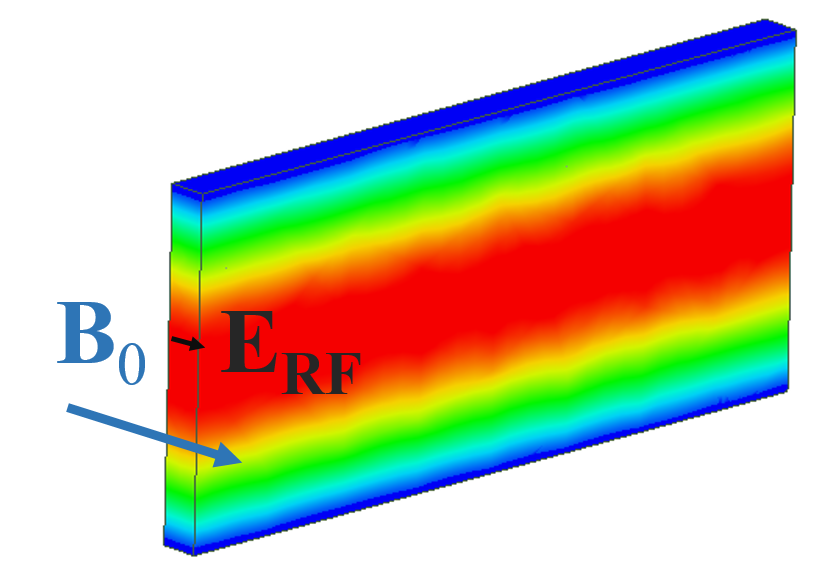
\includegraphics[width=0.9\linewidth]{figures/chap4/rectwg_LH_geometry}
	\caption{Typical geometry of a LHRF antenna thin rectangular waveguide close to the plasma.}
	\label{fig:rectwglhgeometry}
\end{marginfigure}
Near the front face of the antenna, the tokamak string magnetic DC magnetic field (few Teslas) is mostly parallel to the RF electric field in the antenna’s waveguides (Figure~\ref{fig:rectwglhgeometry}), with a strong negative gradient (1 to 2 T/m) along the waveguide longitudinal direction. Multipactor simulations showed a ~7\% reduction of the multipactor electric field threshold with respect to no magnetic field case for narrow waveguides (height<15~mm), as illustrated in Figure~\ref{fig:rectwglhgeometry}. Moreover, strong resonance correlated with the increase of the multipactor order is numerically observed when the total magnetic field (in norm) is such that the electron cyclotron frequency equals the wave frequency. In this case, the multipactor threshold is decreased more strongly for larger waveguides (-60\%) than for narrower ones (-20\%). Such case can lead to ease the breakdown occurrence, a situation which has been experimentally observed on smaller machines for which this range of magnetic field was met at the location of the grill antennas \sidecite[+3cm]{knowlton1982}. Such limitation is generally not observed experimentally on larger machine, due to the fact that the resonance layer occur in much wider waveguides. 

When a magnetic field is directed along the waveguide’s large side direction, i.e. in the poloidal direction ($B_y$), the calculated multipactor power threshold can increase or decrease with respect to the threshold without DC magnetic field. However, in the typical range of radial magnitude observed in tokamak ($B_x$ ~0.1 to 0.3~T, no multipactor occurs. The addition of this $B_y$ field to a $B_0$ component has no effect on the threshold, unless $B_y ~ B_0$ where it is enhanced. 

Finally, the multipactor threshold scales almost linearly with the frequency \sidecite{goniche2014}.


\begin{figure*}[h]
	\centering
	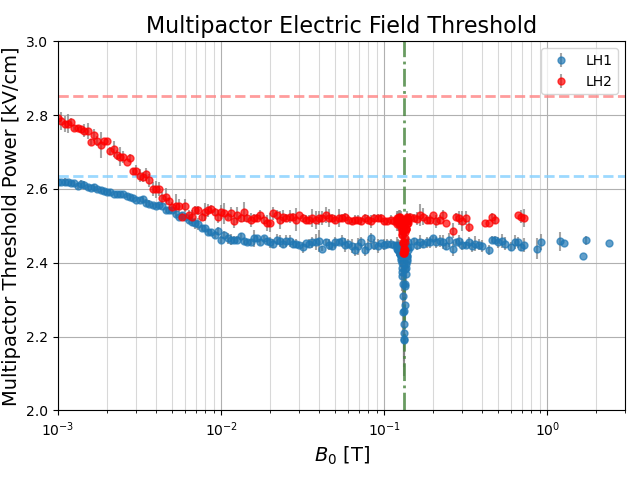
\includegraphics[width=0.48\linewidth]{figures/chap4/Eth_vs_By_C3-C4}
	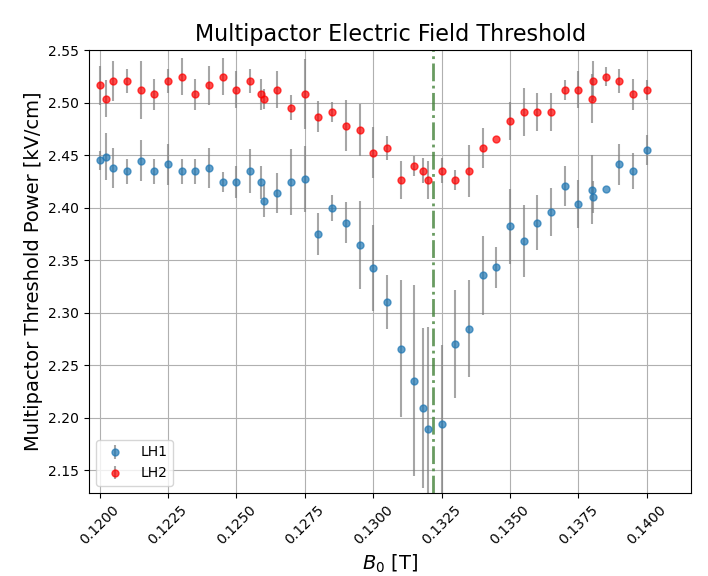
\includegraphics[width=0.48\linewidth]{figures/chap4/Eth_vs_By_C3-C4_zoom}
	\caption{Left: Multipactor electric field threshold for the thin rectangular waveguides of the WEST LH1 and LH2 antennas (70x8mm for LH1 and 76x14.65mm for LH2) at 3.7~GHz versus magnitude of the DC magnetic field $B_0$ parallel to the electric field. Right: zoom for $B_0$ in [$0.12,0.14$T]. Dashed lines are the multipactor threshold without magnetic field. Green dot-dashed vertical line corresponds to cyclotron resonance magnetic field. SEY from Spark3D ECSS Copper.}
	\label{fig:ethvsbyc3-c4}
\end{figure*}

% ###########################################################
% ###########################################################
% ###########################################################
\subsection[Influence of electron emission]{Influence of the secondary emission on multipactor calculations}\label{sec:multipactor_TEEY}
The previous results obtained from multipactor modelling codes always had to assume a specific metal secondary emission properties. When an incident electron (IE) impacts the components' walls, it can penetrate the material and then transfer a part of its energy through inelastic interactions. The IE can excite the inner material electron which could escape the material surface, which is called \textit{secondary electron} (SE). The IE can also escape the surface material due to several inelastic and elastic interactions: in this case the electron emitted is called the \textit{back-scattered electrons} (BSE). We commonly define three yields: 
\begin{itemize}
	\item the Total Electron Emission Yield (TEEY, $\sigma$) which is the number of the whole electrons emitted by the surface divided by the number of IE,
	\item the Secondary-Electron Yield (SEY, $\delta$) which is the number of SE emitted divided by the number of IE,
	\item Back-Scattered Electron Yield (BSEY, $\eta$) which is the
	number of BSE emitted divided by the number of IE. 
\end{itemize}
TEEY is the total of the SEY and the BSEY, i.e. $\sigma=\eta+\delta$. These values depends of the incident electron angle and energy\sidecite[-1cm]{shih1997}, but also on the material temperature \sidecite[-1cm]{belhaj2015}, morphology (defects, roughness, etc.) \sidecite[-0.5cm]{balcon2012} and history (contaminated, cleaned) \sidecite{fil2016}. Moreover, as seen in next Section, it has been shown to depend as well on the local magnetic field \sidecite{fil2017}. A  typical variation of the SEY with the incident energy is shown in Figure~\ref{fig:teeycuexample}. The energy levels for which $\sigma=1$ ($E_{c1}$ and $E_{c2}$) are called first and second \textit{crossover points}. The TEEY reaches a maximum $\sigma_{\max}$ at the energy $E_{\max}$. 

\begin{figure}[h]
	\centering
	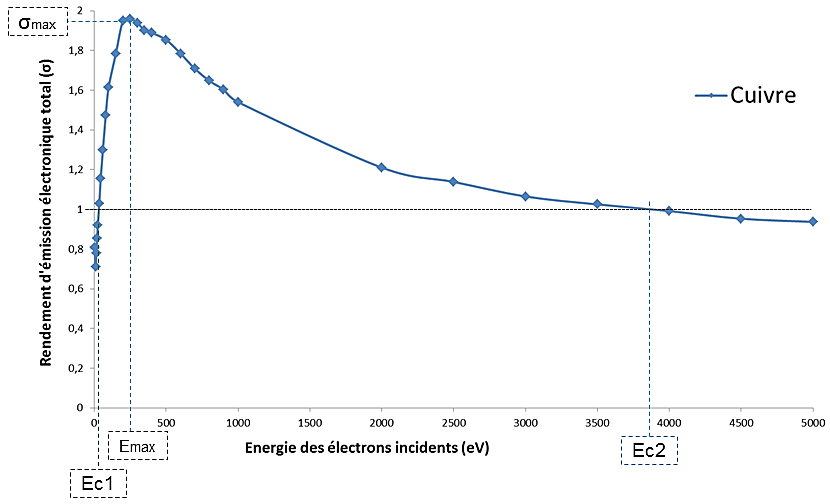
\includegraphics[width=1.0\linewidth]{figures/chap4/TEEY_Cu_example}
	\caption{Example of a TEEY as a function of the incident electron energy for a copper sample (From \citeauthyear{fil2017-1}).}
	\label{fig:teeycuexample}
\end{figure}

It is known from long that the triggering of multipactor depends on the first cross-over energy  $E_{c1}$ and the maximum value of the TEEY curve ($\sigma_{\max}$) \sidecite{kishek1998}. However, as by shown in \citeauthyear{fil2016}, the magnitude of the calculated threshold also heavily depends on the shape of this curve, notably between $E_{c1}$ and $\sigma_{\max}$. Using secondary emission data for silver collected in the literature and experimental multipactor results, Nicolas Fils has shown during his PhD that in order for multipactor simulations to get results close experimental ones, the TEEY model curves need to be accurate in particular between $E_{c1}$ and $E_{\max}$. Hence, for multipactor simulations to be predictive, the TEEY properties of a RF device materials should be well known and representative of the operating conditions such as temperature and surface state. As the later evolves in time due to a combination of multiple factors such as impurity contamination, RF conditioning, breakdowns, prediction of the absolute multipactor threshold is possible but challenging for tokamak RF antennas.

% ###########################################################
% ###########################################################
% ###########################################################
\subsection[Influence of Magnetic Field]{Influence of Magnetic Field on Secondary Emission}\label{sec:multipactor_magnetic_field}
In some applications concerned by the multipactor effect, RF components are subjected to DC magnetic fields. For instance, in telecommunication satellite, magnetic fields of a few tenths of Tesla produced with permanent magnets are used in circulators and isolators. In fusion reactors, rectangular copper waveguides or coaxial transmission lines are located under intense magnetic fields of few Tesla generated by toroidal and poloidal coils. Any externally applied magnetic field will affect charged particle trajectories in inducing a gyro-motion, which in returns is changing the multipactor resonance dynamics. Some simulations and experimental results have  shown that multipactor discharges could even be suppressed in the presence of a constant magnetic field perpendicular to the alternating field in parallel-plate geometries \sidecite{deb1964, geng1999, becerra2007}. However, the effect DC magnetic field on the electron emission process itself was not investigated to our knowledge.

For this reason, a new experimental setup has been developed in the frame of the PhD thesis of Nicolas Fil \sidecite{fil2017-1}. A vacuum chamber of 34~$\si{mm^3}$ has been equipped with a 41~\si{mm}-diameter copper solenoid coil. A 10~\si{mm} disc sample is located as close as possible of the coil in the region where the magnetic field is constant and perpendicular to sample surface. 


\begin{figure}[h]
	\centering
	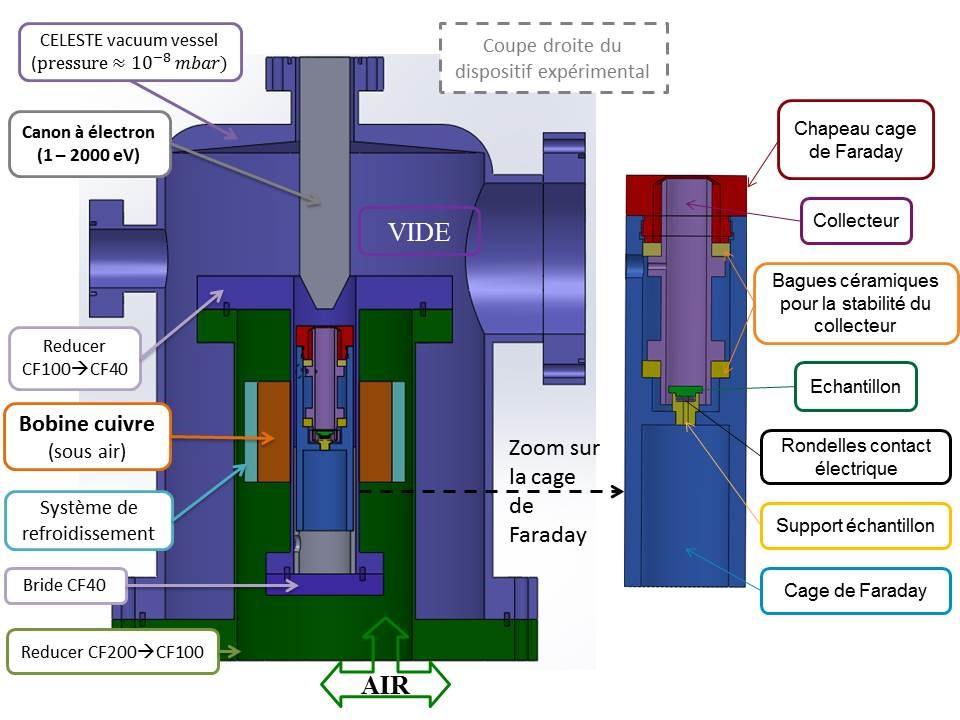
\includegraphics[width=1.0\linewidth]{figures/chap4/CELESTE_magnetic_field}
	\caption{Illustration of the measurement device made in the CELESTE setup at ONERA in \citeauthyear{fil2017-1}.}
	\label{fig:celestemagneticfield}
\end{figure}

TEEY measurements under magnetic fields on three copper samples with different surface morphology have been made \sidecite{fil2018}. Results are reported in Figure~\ref{fig:teeycumagneticfield}. Sample 
"N" has been chosen among a batch of twenty laminate copper samples. This sample has not received
any other treatment except a cleaning process common to all samples. From the same batch, he took other samples on which he applied mechanical polishing with 1~\si{\micro m} abrasive grains. This kind of polishing on copper creates a strain hardening layer near the surface. To clean this layer, a further surface polishing by vibrations has been applied. An additional copper sample given by CERN which have been polished with an electrochemical process has also been measured. 

TEEY has been measured for the three samples under uniform DC magnetic field perpendicular to the macroscopic surface with incident electron. As the multipactor power threshold highly depends on the TEEY at $E_{c1}$, results reported in Figure~\ref{fig:teeycumagneticfield} have been made at the first cross-over energy ($E_{c1}$) (previously measured without magnetic field). TEEY with magnetic field has been found lower than the TEEY without for the three samples. In addition, TEEY of sample N is reduces by 45\% with magnetic field amplitude while TEEY of sample J is weakly influenced by these magnetic fields (decrease to 5\%). This difference indicates that the polishing treatment has reduced the influence of magnetic fields on TEEY. TEEY decreases and then increases with the magnetic field amplitude increasing for all samples. The TEEY minimums are reached at 28.3 mT, 16.98 mT and 11.32 mT respectively for sample N, J and CERN. 

\begin{marginfigure}
	\centering
	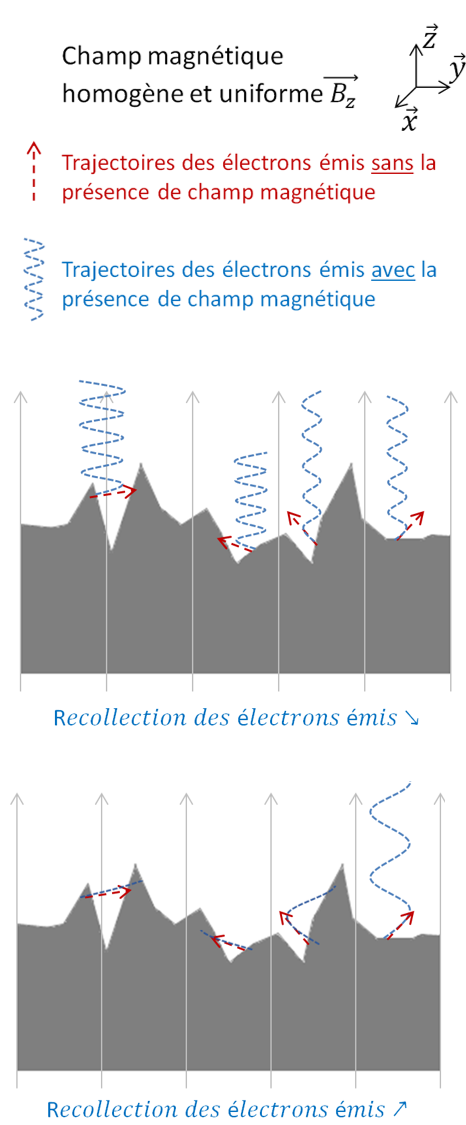
\includegraphics[width=1.0\linewidth]{figures/chap4/electron_trajectory}
	\caption{Schematic of the interpretation of the results. As the amplitude of the magnetic field increases, it reduces the Larmor radius of the electrons trajectories and then decreases the probability of recollection.}
	\label{fig:electrontrajectory}
\end{marginfigure}

The samples surface morphologies has been measured are results are reported in the Table below. The effect of DC magnetic field perpendicular to the surface is weak for polished sample. But if the surface in not polished such as sample N, the magnetic field has a larger effect on the TEEY and then on multipactor threshold. Decreasing the TEEY at first cross-over energy would increase the multipactor threshold \cite{fil2016}, which would increase the transmitted power and the performance of the RF systems limited by the multipactor phenomenon which finally would be a positive effect for many applications.

The results are interpreted as the following. The magnetic field magnitude modifies the emitted electron cyclotron motion, affecting their Larmor radius and therefore their probability to be recollected by the surface (Figure~\ref{fig:electrontrajectory})\footnote{The impact of the magnetic field amplitudes (up to hundreds \si{\milli T}) on the electron trajectories inside the materials is negligible because the mean free paths of electrons of few electron-volts in solids is at least five orders of magnitude smaller than the electron cylindrical helix trajectory dimensions due to the magnetic field. It means that an electron inside the materials would interact with material elements (electrons, nucleus, plasmons) before having his trajectory modified by the magnetic field.}. Hence, the higher the surface features are, the higher the magnetic field amplitude has to be for emitted electrons to escape the surface.

\begin{tabular}{|c|c|c|c|}
	\hline
	Sample &  Surface treatment & Height $R_c$ ($\si{\micro m}$) & Width PSm ($\si{\micro m}$) \\
	\hline
	N & As Received (Laminate) & 1.117 $\pm$ 0.080 & 27.606 $\pm$ 2.874 \\
	\hline
	J & 1\si{\micro m} mechanical polishing & 0.231 $\pm$ 0.011 & 6.565 $\pm$ 0.615 \\
	\hline
	CERN & Electro-polishing &  0.156 $\pm$ 0.012 & 71.767 $\pm$ 9.311 \\
	\hline
\end{tabular}

\begin{figure*}
	\centering
	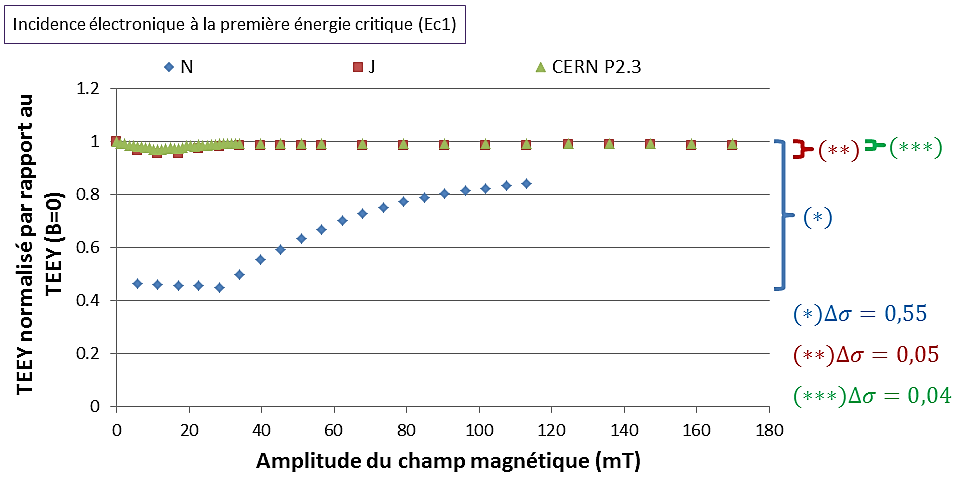
\includegraphics[width=1.0\linewidth]{figures/chap4/TEEY_Cu_magnetic_field}
	\caption{TEEY under magnetic field normalised with TEEY without magnetic field. Incident electron energy at first cross-over energy ($E_{c1}$). Magnetic field normal to the macroscopic surface of the samples. TEEY of three samples (J: polished ; N: non-polished ; CERN sample: electro-polished). (from \citeauthyear{fil2018}).}
	\label{fig:teeycumagneticfield}
\end{figure*}


% ###########################################################
% ###########################################################
% ###########################################################
\subsection[Influence of Dielectric]{Multipactor with dielectric materials} \label{sec:multipactor_dielectric}
\marginnote{The section discusses preliminary results, as the PhD of Adrien Plaçais is not terminated at the time of the writing of this manuscript.}
As discussed in previous Sections, dielectric material are found in RF heating systems, such as RF vacuum windows or as support structures of the coaxial inner conductors.  Dielectrics are also often used inside satellite payloads, as multiplexing filters downstream the High Power Amplifier, or as they enable to lower the equipment size while maintaining the overall electric performances \sidecite{puech2017}. 


\begin{marginfigure}
	\centering
	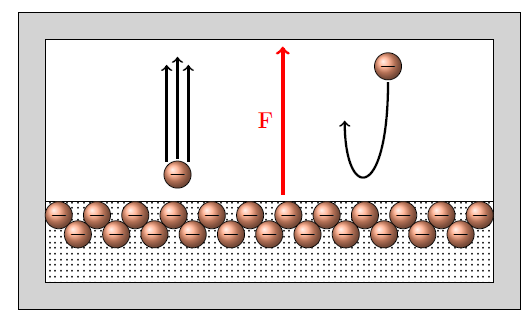
\includegraphics[width=1.0\linewidth]{figures/chap4/dielectric_electrical_charge_effect}
	\caption{Influence of the dielectric charge to electron trajectories (from \citeauthyear{placais2020}).}
	\label{fig:dielectricelectricalchargeeffect}
\end{marginfigure}

In contrary to metals, dielectrics can trap a net electrical charge, which influences the electrons trajectory and thus the multipactor resonance conditions. Moreover, dielectrics electron emission properties vary with their charge. It means that multipactor calculation has to take into account the dynamic aspect of the electron emission properties of dielectric components \sidecite[+2cm]{sorolla2017}. For this reason, a new simulation code called POTOMAC (Physical simulatiOn TOol for Multipactor in Advanced Configurations) has been developed to model this kind of systems in the frame of the PhD of Adrien Plaçais \sidecite[+1cm]{placais2018}. POTOMAC is Particle-In-Cell (PIC) code which is able to take into account the dynamic evolution of the electron emission. 

An important work has been made in POTOMAC to describe material electron emission properties, as function of the incident electron energy and angle, the dielectric charge and keeping tracks of the underlying physical mechanisms and reproducing correctly experimental results \sidecite{placais2018, placais2020-1}. As a general trend, the increase of the dielectric surface charge (negative or positive) increases the multipactor threshold. These preliminary results must be confirmed by further modelling work as well as by experimental results expected from parallel test campaigns.



